\section{CT Block Diagrams}

\subsection{The Four Basic Motifs}

Understanding complex systems, with many interconnections, is aided by graphical representations, generally called block diagrams \footnote{There is a closely related graphical approach called \emph{signal flow graphs} that you may learn about in upper-level courses. They are equivalent to block diagrams, but are more amenable to computer representation and manipulation.}. They are a hybrid graphical-analytical approach.

There are just four basic motifs needed to build any block diagram. Let $\mathcal{S}_i$ denote a (sub) system. Then the four motifs are:

\begin{itemize}
\item A single block.\\[1em] 
\begin{tikzpicture}[auto, node distance=2cm,>=latex',scale=1, every node/.style={transform shape}]
    % We start by placing the blocks
    \node [input, name=input] {};
    \node [block, right of=input] (system) {$\mathcal{S}_1$};
    \node [output, right of=system] (output) {};

    % Once the nodes are placed, connecting them is easy. 
    \draw [draw,->] (input) -- node {$x(t)$} (system);
    \draw [->] (system) -- node {$y(t)$} (output);
\end{tikzpicture}

\item A {\it series} connection of two blocks\\[1em]
\begin{tikzpicture}[auto, node distance=2cm,>=latex',scale=1, every node/.style={transform shape}]
    % We start by placing the blocks
    \node [input, name=input] {};
    \node [block, right of=input] (system1) {$\mathcal{S}_1$};
    \node [block, right of=system1,node distance=4cm] (system2) {$\mathcal{S}_2$};
    \node [output, right of=system2] (output) {};

    % Once the nodes are placed, connecting them is easy. 
    \draw [draw,->] (input) -- node {$x(t)$} (system1);
    \draw [->] (system1) -- (system2);
    \draw [->] (system2) -- node {$y(t)$} (output);
\end{tikzpicture}
\item A {\it parallel} connection of two blocks\\[1em]
\begin{tikzpicture}[auto, node distance=2cm,>=latex',scale=1, every node/.style={transform shape}]
    % We start by placing the blocks and inputs
    \node[shape=coordinate] at (1,1) (input1) {};
    \node[block] at (3,1) (block1) {$\mathcal{S}_1$};
    \node[shape=coordinate] at ($(block1.east)+(0.5,0)$) (output1) {};
    \draw[->] (input1) -- (block1);
    \draw (block1) -- (output1);

    \node[shape=coordinate] at (1,-1) (input2) {};
    \node[block] at (3,-1) (block2) {$\mathcal{S}_2$};
    \node[shape=coordinate] at ($(block2.east)+(0.5,0)$) (output2) {};
    \draw[->] (input2) -- (block2);
    \draw (block2) -- (output2);

    \node [input, name=input] at (0,0) {};  	
    \node [input, name=conn] at (1,0) {};
    \draw (conn) -- (input1);
    \draw (conn) -- (input2);
    \node [sum, right of=input,node distance=5cm] (sum) {$\Sigma$};
    \draw [->] (output1) -| (sum);
    \draw [->] (output2) -| (sum);

    \draw [draw] (input) -- node {$x(t)$} (conn);
    \node [output, right of=sum] (output) {};
    \draw [->] (sum) -- node {$y(t)$} (output);
\end{tikzpicture}

\item A {\it feedback} connection\\[1em]
\begin{tikzpicture}[auto, node distance=2cm,>=latex',scale=1, every node/.style={transform shape}]
    % We start by placing the blocks
    \node[block] at (4,0) (block1) {$\mathcal{S}_1$};

    \node[block] at (4,-2) (block2) {$\mathcal{S}_2$};
    \node[shape=coordinate] at (6,-2) (input2) {};

    \node [input, name=input] at (0,0) {};  	
    \node [shape=coordinate, name=conn] at (6,0) {};
    \draw (block1) -- (conn);
    \draw (conn) -- (input2);
    \draw [->] (input2) -- (block2);

    \node [sum, right of=input,node distance=2cm] (sum) {$\Sigma$};
    \draw [->] (block2) -| node[pos=0.95] {$-$} (sum);

    \draw [draw,->] (input) -- node {$x(t)$} (sum);
    \draw [->] (sum) -- (block1);
    \node [output, right of=conn] (output) {};
    \draw [->] (conn) -- node {$y(t)$} (output);
\end{tikzpicture}
\end{itemize}

Note the feedback is negative (the minus sign on the feedback summation input). These can be use in various combinations, as we shall see shortly.

\subsection{Connections to Convolution}

Each subsystem, $\mathcal{S}_i$, can be represented by a basic time-domain operation (e.g. derivatives, integrals, addition, and scaling) or more generally by it's impulse response $h_i(t)$.
\
For example a block representing an system acting as integrator is typically drawn as

\begin{center}
  \begin{tikzpicture}[auto, node distance=2cm,>=latex',scale=1, every node/.style={transform shape}]
    % We start by placing the blocks
    \node [input, name=input] {};
    \node [block, right of=input] (system) {$\int$};
    \node [output, right of=system] (output) {};

    % Once the nodes are placed, connecting them is easy. 
    \draw [draw,->] (input) -- node {$x(t)$} (system);
    \draw [->] (system) -- node[pos=3] {$y(t) = \int\limits_{-\infty}^t x(\tau) \; d\tau$} (output);
\end{tikzpicture}
\end{center}
This is equivalent to an impulse response $h(t) = u(t)$ so that it might also be drawn as
\begin{center}
  \begin{tikzpicture}[auto, node distance=2cm,>=latex',scale=1, every node/.style={transform shape}]
    % We start by placing the blocks
    \node [input, name=input] {};
    \node [block, right of=input] (system) {$h(t) = u(t)$};
    \node [output, right of=system] (output) {};

    % Once the nodes are placed, connecting them is easy. 
    \draw [draw,->] (input) -- node {$x(t)$} (system);
    \draw [->] (system) -- node[pos=3] {$y(t) = x(t) * u(t) = \int\limits_{-\infty}^t x(\tau) \; d\tau$} (output);
\end{tikzpicture}
\end{center}

We can use the concept of convolution to connect block diagrams to the properties of convolution

\begin{itemize}
\item A single block is equivalent to convolution with the impulse response for that subsystem\\[1em] 
\begin{tikzpicture}[auto, node distance=2cm,>=latex',scale=1, every node/.style={transform shape}]
    % We start by placing the blocks
    \node [input, name=input] {};
    \node [block, right of=input] (system) {$h_1(t)$};
    \node [output, right of=system] (output) {};

    % Once the nodes are placed, connecting them is easy. 
    \draw [draw,->] (input) -- node {$x(t)$} (system);
    \draw [->] (system) -- node[pos=2] {$y(t) = h_1(t)*x(t)$} (output);
\end{tikzpicture}

\item Using the associative property, a series connection of two blocks becomes
  \begin{center}
\begin{tikzpicture}[auto, node distance=2cm,>=latex',scale=1, every node/.style={transform shape}]
    % We start by placing the blocks
    \node [input, name=input] {};
    \node [block, right of=input] (system1) {$h_1(t)$};
    \node [block, right of=system1,node distance=4cm] (system2) {$h_2(t)$};
    \node [output, right of=system2] (output) {};

    \draw [draw,->] (input) -- node {$x(t)$} (system1);
    \draw [->] (system1) -- (system2);
    \draw [->] (system2) -- node[pos=3] {$y(t) = \left[h_1(t)*h_2(t)\right]*x(t)$} (output);
\end{tikzpicture}
  \end{center}
  which can be reduced to a single convolution $y(t) = h_3(t)*x(t)$ where $h_3(t) = h_1(t)*h_2(t)$.
\item Using the distributive property, a parallel connection of two blocks becomes
  \begin{center}
\begin{tikzpicture}[auto, node distance=2cm,>=latex',scale=1, every node/.style={transform shape}]

    \node[shape=coordinate] at (1,1) (input1) {};
    \node[block] at (3,1) (block1) {$h_1(t)$};
    \node[shape=coordinate] at ($(block1.east)+(0.5,0)$) (output1) {};
    \draw[->] (input1) -- (block1);
    \draw (block1) -- (output1);

    \node[shape=coordinate] at (1,-1) (input2) {};
    \node[block] at (3,-1) (block2) {$h_2(t)$};
    \node[shape=coordinate] at ($(block2.east)+(0.5,0)$) (output2) {};
    \draw[->] (input2) -- (block2);
    \draw (block2) -- (output2);

    \node [input, name=input] at (0,0) {};  	
    \node [input, name=conn] at (1,0) {};
    \draw (conn) -- (input1);
    \draw (conn) -- (input2);
    \node [sum, right of=input,node distance=5cm] (sum) {$\Sigma$};
    \draw [->] (output1) -| (sum);
    \draw [->] (output2) -| (sum);

    \draw [draw] (input) -- node {$x(t)$} (conn);
    \node [output, right of=sum] (output) {};
    \draw [->] (sum) -- node[pos=3] {$y(t)= \left[h_1(t)*x(t)\right] +  \left[h_2(t)*x(t)\right] =  \left[h_1(t)+h_2(t)\right]*x(t)$} (output);
\end{tikzpicture}  
  \end{center}
  which is equivalent to a single convolution $y(t) = h_3(t)*x(t)$ where $h_3(t) = h_1(t) + h_2(t)$.
\item In the feedback connection let $w(t)$ be the output of the summation
  \begin{center}
\begin{tikzpicture}[auto, node distance=2cm,>=latex',scale=1, every node/.style={transform shape}]
    % We start by placing the blocks
    \node[block] at (4.5,0) (block1) {$h_1(t)$};

    \node[block] at (4,-2) (block2) {$h_2(t)$};
    \node[shape=coordinate] at (6,-2) (input2) {};

    \node [input, name=input] at (0,0) {};  	
    \node [shape=coordinate, name=conn] at (6,0) {};
    \draw (block1) -- (conn);
    \draw (conn) -- (input2);
    \draw [->] (input2) -- (block2);

    \node [sum, right of=input,node distance=2cm] (sum) {$\Sigma$};
    \draw [->] (block2) -| node[pos=0.95] {$-$} (sum);

    \draw [draw,->] (input) -- node {$x(t)$} (sum);
    \draw [->] (sum) -- (block1);
    \node [output, right of=conn] (output) {};
    \draw [->] (conn) -- node {$y(t)$} (output);
    \draw node at (3,0.3) {$w(t)$};
\end{tikzpicture}
  \end{center}
  Then $y(t) = h_1(t)*w(t)$ and $w(t) = x(t) - h_2(t)*y(t)$. Substituting the later into the former gives $y(t) = h_1*(x-h_2(t)*y(t))$. Using the distributive property we get $y(t) = h_1(t)*x(t) - h_1(t)*h_2(t)*y(t)$. Isolating the input on the right-hand side and using $y(t) = \delta(t)*y(t)$ we get
  \[
  y(t) + h_1(t)*h_2(t)*y(t) = \left[\delta(t) + h_1(t)*h_2(t)\right]*y(t) = h_1(t)*x(t) 
  \]
  We can solve this for $y(t)$ using the concept of inverse systems. Let $h_3(t)* \left[\delta(t) + h_1(t)*h_2(t)\right]= \delta(t)$, i.e. $h_3$ is the inverse system of $\delta(t) + h_1(t)*h_2(t)$. Then
  \[
  y(t) = h_3(t)*h_1(t)*x(t)
  \]
\end{itemize}

Recall, when the system is instantaneous (memoryless) the impulse response is $a\delta(t)$ for some constant $a$. This is the same as scaling the signal by $a$. We typically drop the block in such cases and draw the input-output operation as

\begin{center}
\begin{tikzpicture}[auto, node distance=2cm,>=latex',scale=1, every node/.style={transform shape}]
  \node [input, name=input] at (0,0) {};
  \node [output, name=system] at (2,0) {};
  \node [output, name=output] at (4,0) {};
  \draw [draw,->] (input) -- node {$x(t)$} (system);
  \draw [draw,->] (system) -- node[pos=1] {$y(t) = ax(t)$} (output);
  \draw [->] (input) -- node {$a$} (output);
\end{tikzpicture}
\end{center}

These properties allow us to perform transformations, either breaking up a system into subsystems, or reducing a system to a single block.

\begin{example}
  Consider a second-order system system with impulse response
  \[
  h(t) = \left(e^{-3t} - e^{-t}\right)\, u(t)
  \]
  We can express this as a block diagram consisting of two parallel blocks
  \begin{center}
\begin{tikzpicture}[auto, node distance=2cm,>=latex',scale=1, every node/.style={transform shape}]

    \node[shape=coordinate] at (1,1) (input1) {};
    \node[block] at (3,1) (block1) {$h_1(t) = e^{-3t}u(t)$};
    \node[shape=coordinate] at ($(block1.east)+(0.5,0)$) (output1) {};
    \draw[->] (input1) -- (block1);
    \draw (block1) -- (output1);

    \node[shape=coordinate] at (1,-1) (input2) {};
    \node[block] at (3,-1) (block2) {$h_2(t) = -e^{-t}u(t)$};
    \node[shape=coordinate] at ($(block2.east)+(0.5,0)$) (output2) {};
    \draw[->] (input2) -- (block2);
    \draw (block2) -- (output2);

    \node [input, name=input] at (0,0) {};  	
    \node [input, name=conn] at (1,0) {};
    \draw (conn) -- (input1);
    \draw (conn) -- (input2);
    \node [sum, right of=input,node distance=5cm] (sum) {$\Sigma$};
    \draw [->] (output1) -| (sum);
    \draw [->] (output2) -| (sum);

    \draw [draw] (input) -- node {$x(t)$} (conn);
    \node [output, right of=sum] (output) {};
    \draw [->] (sum) -- node[pos=1] {$y(t)$} (output);
\end{tikzpicture}
  \end{center}

\end{example}

\begin{example}
  Consider a system with block diagram

  \begin{center}
\begin{tikzpicture}[auto, node distance=2cm,>=latex',scale=1, every node/.style={transform shape}]

    \node[shape=coordinate] at (1,1) (input1) {};
    \node[block] at (3,1) (block1) {$h_1(t) = e^{-2t}u(t)$};
    \node[shape=coordinate] at ($(block1.east)+(0.5,0)$) (output1) {};
    \draw[->] (input1) -- (block1);
    \draw (block1) -- (output1);

    \node[shape=coordinate] at (1,-1) (input2) {};
    \node[block] at (3,-1) (block2) {$h_2(t) = -e^{-4t}u(t)$};
    \node[shape=coordinate] at ($(block2.east)+(0.5,0)$) (output2) {};
    \draw[->] (input2) -- (block2);
    \draw (block2) -- (output2);

    \node[block] at (8,0) (block3) {$h_3(t) = e^{-6t}u(t)$};

    \node [input, name=input] at (0,0) {};  	
    \node [input, name=conn] at (1,0) {};
    \draw (conn) -- (input1);
    \draw (conn) -- (input2);
    \node [sum, right of=input,node distance=5cm] (sum) {$\Sigma$};
    \draw [->] (output1) -| (sum);
    \draw [->] (output2) -| (sum);

    \draw [draw] (input) -- node {$x(t)$} (conn);
    \node [output, right of=block3] (output) {};
    \draw [->] (sum) -- (block3);
    \draw [->] (block3) -- node[pos=1] {$y(t)$} (output);
\end{tikzpicture}
  \end{center}
  We can determine the overall impulse response of this system using the distributive and associative properties
\begin{align*}
  h(t) &= \left[ h_1(t) + h_2(t)\right]*h_3(t)\\
  &= h_1(t)*h_3(t) + h_2(t)*h_3(t)\\
  &= \left[ e^{-2t}u(t)\right]*\left[ e^{-6t}u(t)\right] + \left[-e^{-4t}u(t) \right]*\left[ e^{-6t}u(t)\right]
\end{align*}
Using the convolution table from Lecture 8 we get the overall impulse response
\[
h(t) = \frac{e^{-2 t}-e^{-6 t}}{4}u(t) - \frac{e^{-4 t}-e^{-6 t}}{2}u(t) = \frac{1}{4}e^{-2t}u(t) -\frac{1}{2}e^{-4t}u(t) + \frac{1}{4}e^{-6t}u(t)
\]
\end{example}


\subsection{Connections to LCCDE}

The other system representation we have seen are linear, constant-coefficient differential equations. These can be expressed as combinations of derivative and/or integration blocks.

\subsubsection*{First-Order System}

To illustrate this consider the first-order LCCDE
\[
\frac{dy}{dt}(t) + ay(t) = x(t)
\]
We can solve this for $y(t)$
\[
y(t) = -\frac{1}{a} \frac{dy}{dt}(t) + \frac{1}{a}x(t)
\]
and can express this as a feedback motif
\begin{center}
  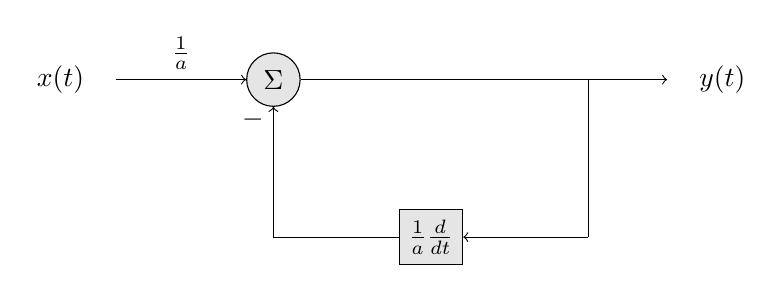
\begin{tikzpicture}[auto]
    \node[block] at (4,-2) (block2) {$\frac{1}{a}\frac{d}{dt}$};
    \node[shape=coordinate] at (6,-2) (input2) {};
    \node [input, name=input] at (0,0) {};  	
    \node [shape=coordinate, name=conn] at (6,0) {};
    \node [sum, right of=input,node distance=2cm] (sum) {$\Sigma$};
    
    \draw (sum) -- (conn);
    \draw (conn) -- (input2);
    \draw [->] (input2) -- (block2);
    \draw [->] (block2) -| node[pos=0.95] {$-$} (sum);
    \draw [draw,->] (input) -- node {$\frac{1}{a}$} (sum);
    \node [left of=input, node distance=2em] {$x(t)$};
    \node [output, right of=conn] (output) {};
    \draw [->] (conn) -- (output);
    \node [right of=output, node distance=2em] {$y(t)$}; 
\end{tikzpicture}
\end{center}

Alternatively we could integrate the differential equation
\begin{align*}
  \frac{dy}{dt}(t) + ay(t) &= x(t)\\
  \int\limits_{-\infty}^t \frac{dy}{dt}(\tau)\; d\tau + a\int\limits_{-\infty}^t y(\tau)\; d\tau &= \int\limits_{-\infty}^t x(\tau)\; d\tau\\
  y(\tau) \Big|_{-\infty}^t  + a\int\limits_{-\infty}^t y(\tau)\; d\tau &= \int\limits_{-\infty}^t x(\tau)\; d\tau\\
\end{align*}
Under the assumption $y(-\infty) = 0$ we can solve this for $y(t)$ to get
\[
  y(t) = -a\int\limits_{-\infty}^t y(\tau)\; d\tau + \int\limits_{-\infty}^t x(\tau)\; d\tau
\]
which can be expressed as the block diagram
\begin{center}
  \tikzstyle{block} = [draw, fill=gray!20, rectangle, 
    minimum height=2em, minimum width=2em]
  \tikzstyle{sum} = [draw, fill=gray!20, circle, node distance=1cm]
  \tikzstyle{input} = [coordinate]
  \tikzstyle{output} = [coordinate]
  \tikzstyle{pinstyle} = [pin edge={to-,thin,black}]
  
  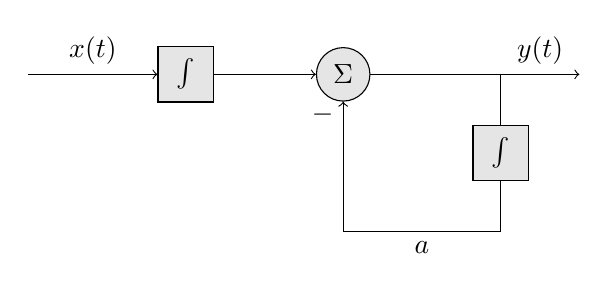
\begin{tikzpicture}[auto]
    \node [input, name=input] at (0,0) {};  	
    \node[block] at (2,0) (block1) {$\int$};
    \node[block] at (6,-1) (block2) {$\int$};
    \node[shape=coordinate] at (6,-2) (input2) {};

    \node [shape=coordinate, name=conn] at (6,0) {};
    \node [shape=coordinate, name=conn2] at (4,-2) {};
    \node [shape=coordinate, name=conn3] at (6,-2) {};
    \node [sum, right of=block1,node distance=2cm] (sum) {$\Sigma$};
    \node [output, right of=conn] (output) {};
    
    \draw (sum) -- (conn);
    \draw (conn) -- (block2);
    \draw (block2) -- (conn3);
    \draw (conn3) -- node {$a$} (conn2);
    \draw [->] (conn2) -| node[pos=0.95] {$-$} (sum);
    \draw [draw,->] (input) -- node {$x(t)$} (block1);
    \draw [->] (block1) -- (sum);
    \draw [->] (conn) -- node {$y(t)$} (output);
  \end{tikzpicture}
\end{center}

We can simplify this block diagram, by noting
\begin{align*}
  y(t) &= -a\int\limits_{-\infty}^t y(\tau)\; d\tau + \int\limits_{-\infty}^t
  x(\tau)\; d\tau\\
  &= \int\limits_{-\infty}^t \left(-a y(\tau) +  x(\tau)\right)\; d\tau\\
\end{align*}
which requires only a single integrator
\begin{center}
  \tikzstyle{block} = [draw, fill=gray!20, rectangle, 
    minimum height=2em, minimum width=2em]
  \tikzstyle{sum} = [draw, fill=gray!20, circle, node distance=1cm]
  \tikzstyle{input} = [coordinate]
  \tikzstyle{output} = [coordinate]
  \tikzstyle{pinstyle} = [pin edge={to-,thin,black}]
  
  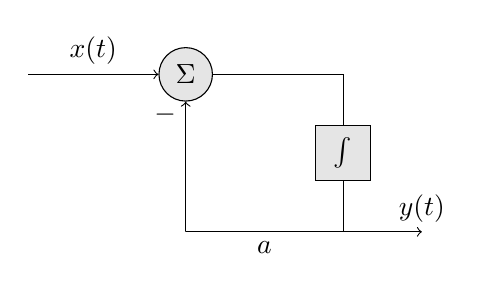
\begin{tikzpicture}[auto]
    \node [input, name=input] at (0,0) {};  	
    \node[block] at (4,-1) (block2) {$\int$};

    \node [shape=coordinate, name=conn] at (4,0) {};
    \node [shape=coordinate, name=conn2] at (2,-2) {};
    \node [shape=coordinate, name=conn3] at (4,-2) {};
    \node [sum, right of=input,node distance=2cm] (sum) {$\Sigma$};
    \node [output, right of=conn3] (output) {};
    
    \draw (sum) -- (conn);
    \draw (conn) -- (block2);
    \draw (block2) -- (conn3);
    \draw (conn3) -- node {$a$} (conn2);
    \draw [->] (conn2) -| node[pos=0.95] {$-$} (sum);
    \draw [draw,->] (input) -- node {$x(t)$} (sum);
    \draw [->] (conn3) -- node[pos=1] {$y(t)$} (output);
  \end{tikzpicture}
\end{center}

The choice of using derivative or integrator blocks is not arbitrary in practice. Derivatives are sensitive to noise at high frequencies (for reasons we will see later in the semester) and so integrators perform much better when implemented in hardware. 

\subsubsection*{Second-Order System}

Now consider the second-order system
\[
\frac{d^2y}{dt^2}(t) + a\frac{dy}{dt}(t)  + by(t)= x(t)
\]
Using a similar process to the first-order system, we can express this as (dropping the limits of integration for clarity):
\[
y(t) = -a \int y(\tau)\; d\tau + \int\int \left( -by(\tau) + x(\tau) \right) \; d\tau^2 
\]
which has the block diagram

\begin{center}
  \tikzstyle{block} = [draw, fill=gray!20, rectangle, 
    minimum height=2em, minimum width=2em]
  \tikzstyle{sum} = [draw, fill=gray!20, circle, node distance=1cm]
  \tikzstyle{input} = [coordinate]
  \tikzstyle{output} = [coordinate]
  \tikzstyle{pinstyle} = [pin edge={to-,thin,black}]
  
  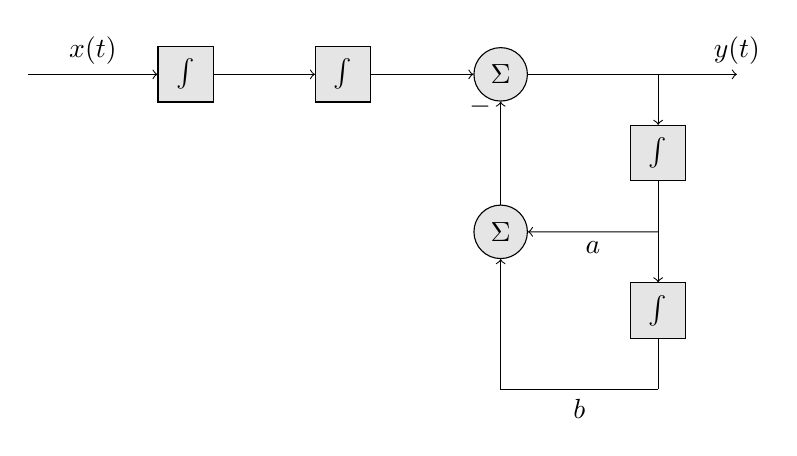
\begin{tikzpicture}[auto]
    \node [input, name=input] at (0,0) {};
    \node [block, right of=input,node distance=2cm] (block1) {$\int$};
    \node [block, right of=block1,node distance=2cm] (block2) {$\int$};
    \node [sum, right of=block2,node distance=2cm] (sum) {$\Sigma$};
    \node [sum, below of=sum,node distance=2cm] (sum2) {$\Sigma$};
    \node[block] at (8,-1) (block3) {$\int$};
    \node[block] at (8,-3) (block4) {$\int$};

    \node [shape=coordinate, name=conn1] at (8,0) {};
    \node [shape=coordinate, name=conn2] at (8,-2) {};
    \node [shape=coordinate, name=conn3] at (8,-4) {};
    \node [shape=coordinate, name=conn4] at (6,-4) {};
    \node [output, right of=conn1] (output) {};

    \draw [->] (input) -- node {$x(t)$} (block1);
    \draw [->] (block1) -- (block2);
    \draw [->] (block2) -- (sum);
    \draw (sum) -- (conn1);
    \draw [->] (conn1) -- (block3);
    \draw (block3) -- (conn2);
    \draw [->] (conn2) -- (block4);
    \draw [->] (conn2) -- node {$a$} (sum2);
    \draw (block4) -- (conn3);
    \draw (conn3) -- node {$b$} (conn4);
    \draw [->] (conn3) -| (sum2);
    \draw [->] (sum2) -- node[pos=0.95] {$-$} (sum);
    \draw [->] (conn1) -- node[pos=1] {$y(t)$} (output);
  \end{tikzpicture}
\end{center}
This is equivalent to two systems in series

\begin{center}
  \tikzstyle{block} = [draw, fill=gray!20, rectangle, 
    minimum height=2em, minimum width=2em]
  \tikzstyle{sum} = [draw, fill=gray!20, circle, node distance=1cm]
  \tikzstyle{input} = [coordinate]
  \tikzstyle{output} = [coordinate]
  \tikzstyle{pinstyle} = [pin edge={to-,thin,black}]
  
  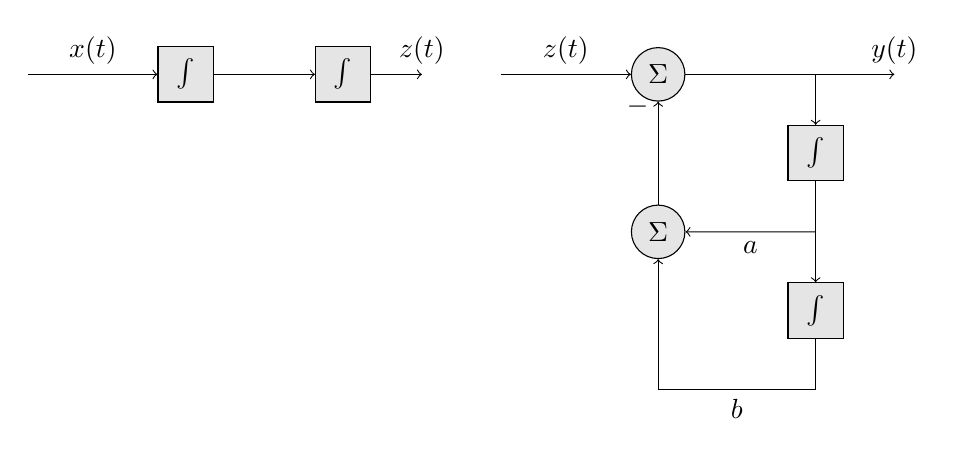
\begin{tikzpicture}[auto]
    \node [input, name=input1] at (0,0) {};
    \node [block, right of=input1,node distance=2cm] (block1) {$\int$};
    \node [block, right of=block1,node distance=2cm] (block2) {$\int$};
    \node [output, right of=block2] (output) {};

    \draw [->] (input1) -- node {$x(t)$} (block1);
    \draw [->] (block1) -- (block2);
    \draw [->] (block2) -- node[pos=1] {$z(t)$} (output);

    \node [input, name=input2] at (6,0) {};
    \node [sum, right of=input2,node distance=2cm] (sum) {$\Sigma$};
    \node [sum, below of=sum,node distance=2cm] (sum2) {$\Sigma$};
    \node[block] at (10,-1) (block3) {$\int$};
    \node[block] at (10,-3) (block4) {$\int$};

    \node [shape=coordinate, name=conn1] at (10,0) {};
    \node [shape=coordinate, name=conn2] at (10,-2) {};
    \node [shape=coordinate, name=conn3] at (10,-4) {};
    \node [shape=coordinate, name=conn4] at (8,-4) {};
    \node [output, right of=conn1] (output) {};

    \draw [->] (input2) -- node {$z(t)$} (sum);
    \draw (sum) -- (conn1);
    \draw [->] (conn1) -- (block3);
    \draw (block3) -- (conn2);
    \draw [->] (conn2) -- (block4);
    \draw [->] (conn2) -- node {$a$} (sum2);
    \draw (block4) -- (conn3);
    \draw (conn3) -- node {$b$} (conn4);
    \draw [->] (conn3) -| (sum2);
    \draw [->] (sum2) -- node[pos=0.95] {$-$} (sum);
    \draw [->] (conn1) -- node[pos=1] {$y(t)$} (output);
    \end{tikzpicture}
\end{center}

Recall that, from the commutative property of convolution, the order of systems in series can be swapped\\

\begin{center}
\tikzstyle{block} = [draw, fill=gray!20, rectangle, 
    minimum height=2em, minimum width=2em]
  \tikzstyle{sum} = [draw, fill=gray!20, circle, node distance=1cm]
  \tikzstyle{input} = [coordinate]
  \tikzstyle{output} = [coordinate]
  \tikzstyle{pinstyle} = [pin edge={to-,thin,black}]
  
  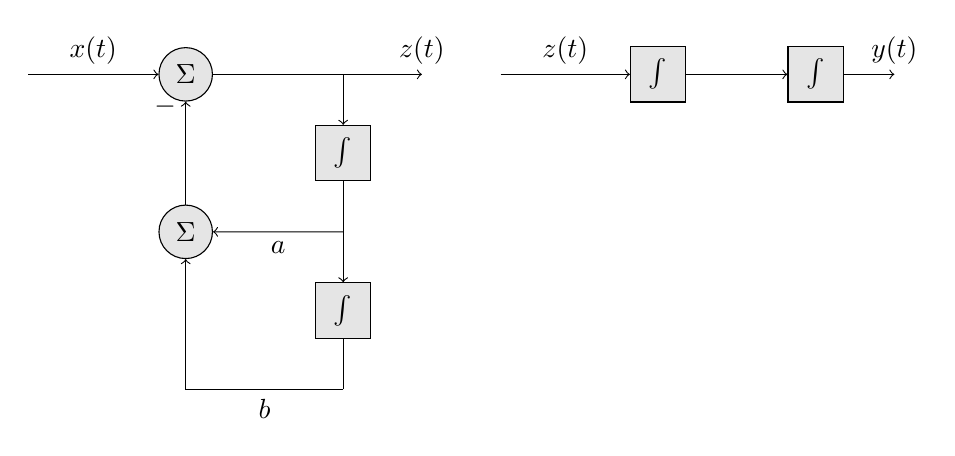
\begin{tikzpicture}[auto]
    \node [input, name=input] at (0,0) {};
    \node [sum, right of=input,node distance=2cm] (sum) {$\Sigma$};
    \node [sum, below of=sum,node distance=2cm] (sum2) {$\Sigma$};
    \node[block] at (4,-1) (block3) {$\int$};
    \node[block] at (4,-3) (block4) {$\int$};

    \node [shape=coordinate, name=conn1] at (4,0) {};
    \node [shape=coordinate, name=conn2] at (4,-2) {};
    \node [shape=coordinate, name=conn3] at (4,-4) {};
    \node [shape=coordinate, name=conn4] at (2,-4) {};
    \node [output, right of=conn1] (output) {};

    \draw [->] (input) -- node {$x(t)$} (sum);
    \draw (sum) -- (conn1);
    \draw [->] (conn1) -- (block3);
    \draw (block3) -- (conn2);
    \draw [->] (conn2) -- (block4);
    \draw [->] (conn2) -- node {$a$} (sum2);
    \draw (block4) -- (conn3);
    \draw (conn3) -- node {$b$} (conn4);
    \draw [->] (conn3) -| (sum2);
    \draw [->] (sum2) -- node[pos=0.95] {$-$} (sum);
    \draw [->] (conn1) -- node[pos=1] {$z(t)$} (output);

    \node [input, name=input] at (6,0) {};
    \node [block, right of=input,node distance=2cm] (block1) {$\int$};
    \node [block, right of=block1,node distance=2cm] (block2) {$\int$};
    \node [output, right of=block2] (output) {};

    \draw [->] (input) -- node {$z(t)$} (block1);
    \draw [->] (block1) -- (block2);
    \draw [->] (block2) -- node[pos=1] {$y(t)$} (output);
  \end{tikzpicture}
\end{center}
We then note that the signal $z$ and the output of the integrator blocks are the same in both systems so that they can be combined into a single block diagram as follows, reducing the number of integrators by two

\begin{center}
  \tikzstyle{block} = [draw, fill=gray!20, rectangle, 
    minimum height=2em, minimum width=2em]
  \tikzstyle{sum} = [draw, fill=gray!20, circle, node distance=1cm]
  \tikzstyle{input} = [coordinate]
  \tikzstyle{output} = [coordinate]
  \tikzstyle{pinstyle} = [pin edge={to-,thin,black}]
  
  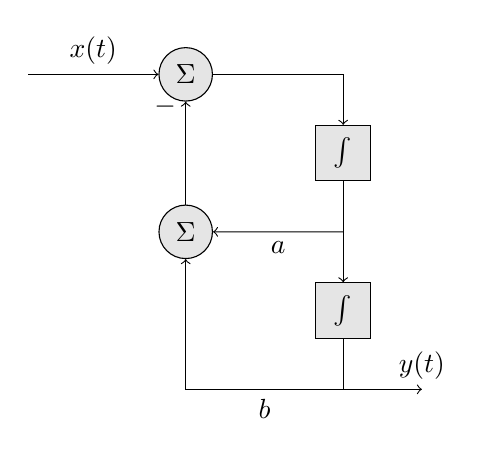
\begin{tikzpicture}[auto]
    \node [input, name=input] at (0,0) {};
    \node [sum, right of=input,node distance=2cm] (sum) {$\Sigma$};
    \node [sum, below of=sum,node distance=2cm] (sum2) {$\Sigma$};
    \node[block] at (4,-1) (block3) {$\int$};
    \node[block] at (4,-3) (block4) {$\int$};

    \node [shape=coordinate, name=conn1] at (4,0) {};
    \node [shape=coordinate, name=conn2] at (4,-2) {};
    \node [shape=coordinate, name=conn3] at (4,-4) {};
    \node [shape=coordinate, name=conn4] at (2,-4) {};
    \node [output, right of=conn3] (output) {};

    \draw [->] (input) -- node {$x(t)$} (sum);
    \draw (sum) -- (conn1);
    \draw [->] (conn1) -- (block3);
    \draw (block3) -- (conn2);
    \draw [->] (conn2) -- (block4);
    \draw [->] (conn2) -- node {$a$} (sum2);
    \draw (block4) -- (conn3);
    \draw (conn3) -- node {$b$} (conn4);
    \draw [->] (conn3) -| (sum2);
    \draw [->] (sum2) -- node[pos=0.95] {$-$} (sum);
    \draw [->] (conn3) -- node[pos=1] {$y(t)$} (output);
  \end{tikzpicture}
\end{center}

\subsection{Implementing a System in Hardware}

One of the most powerful uses of block diagrams is the implementation of a CT system in hardware. As we shall see later in the semester, designing CT systems for a particular purpose leads to a mathematical description that is equivalent to either an impulse response, or a LCCDE. We have seen how these can be represented as block diagrams. Once we have reduced a system to blocks consisting of simple operations, we can then convert the block diagram to a circuit.

\begin{tabular}{cc}

  Block & Typical Circuit\\
  \hline
  \tikzstyle{block} = [draw, fill=gray!20, rectangle, 
    minimum height=2em, minimum width=2em]
  \tikzstyle{sum} = [draw, fill=gray!20, circle, node distance=1cm]
  \tikzstyle{input} = [coordinate]
  \tikzstyle{output} = [coordinate]
  \tikzstyle{pinstyle} = [pin edge={to-,thin,black}]
  
  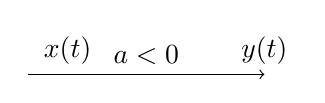
\begin{tikzpicture}[auto]
    \node [input, name=input] at (0,0) {};
    \node [shape=coordinate, name=signal1] at (1,0) {};
    \node [shape=coordinate, name=signal2] at (2,0) {};
    \node [output, right of=signal2] (output) {};

    \draw (input) -- node {$x(t)$} (signal1);
    \draw (signal1) -- node {$a < 0$} (signal2);
    \draw [->] (signal2) -- node[pos=1] {$y(t)$} (output);
  \end{tikzpicture}  

  &
  \begin{circuitikz}[american voltages,scale=0.8, every node/.style={transform shape}]
    \draw
    (5,3.5) node[op amp] (opamp1) {}
    (0,4) to[R,l=$R_1$,o-] (4,4)
    (4,4) to[short] (opamp1.-)
    (opamp1.+) to[short] (3.8,2) 
    (0,2) to[short,o-o] (8,2)
    (opamp1.out) to[short] (6.2,5)
    (3.5,5) to[R,l=$R_2$] (6.2,5)
    (3.5,4) to[short] (3.5,5)
    (opamp1.out) to[short,-o] (8,3.5)
    (0,4) to[open, v=$x(t)$] (0,2)
    (8,3.5) to[open, v=$y(t)$] (8,2);
  \end{circuitikz}
  \\[2em]
  
  \tikzstyle{block} = [draw, fill=gray!20, rectangle, 
    minimum height=2em, minimum width=2em]
  \tikzstyle{sum} = [draw, fill=gray!20, circle, node distance=1cm]
  \tikzstyle{input} = [coordinate]
  \tikzstyle{output} = [coordinate]
  \tikzstyle{pinstyle} = [pin edge={to-,thin,black}]
  
  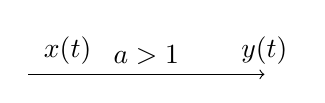
\begin{tikzpicture}[auto]
    \node [input, name=input] at (0,0) {};
    \node [shape=coordinate, name=signal1] at (1,0) {};
    \node [shape=coordinate, name=signal2] at (2,0) {};
    \node [output, right of=signal2] (output) {};

    \draw (input) -- node {$x(t)$} (signal1);
    \draw (signal1) -- node {$a > 1$} (signal2);
    \draw [->] (signal2) -- node[pos=1] {$y(t)$} (output);
  \end{tikzpicture}  
  &
  \begin{circuitikz}[american voltages,scale=0.8, every node/.style={transform shape}]
    \draw
    (7,3.5) node[op amp] (opamp1) {}
    (4,0) to[short,o-o] (12,0)
    (4,4) to[short,o-] (opamp1.-)
    (opamp1.+) to[short] (5.8,1.75)
    (5.8,1.75) to[short] (8.2,1.75)
    (opamp1.out) to[R, l=$R_1$] (8.2,1.75)
    (8.2,1.75) to[R, l=$R_2$] (8.2,0)
    (opamp1.out) to[short, -o] (12,3.5)
    (4,4) to[open, v=$x(t)$] (4,0)
    (12,3.5) to[open, v=$y(t)$] (12,0);
  \end{circuitikz}
  \\[2em]

      \tikzstyle{block} = [draw, fill=gray!20, rectangle, 
        minimum height=2em, minimum width=2em]
      \tikzstyle{sum} = [draw, fill=gray!20, circle, node distance=1cm]
      \tikzstyle{input} = [coordinate]
      \tikzstyle{output} = [coordinate]
      \tikzstyle{pinstyle} = [pin edge={to-,thin,black}]
      
      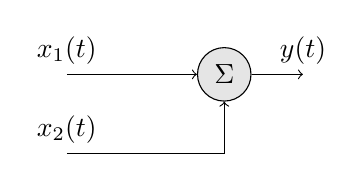
\begin{tikzpicture}[auto]
        \node [input, name=input1] at (0,0) {};
        \node [input, name=input2] at (0,-1) {};
        \node [sum] at (2,0) (sum1) {$\Sigma$};
        \node [output, right of=sum1] (output) {};
        
        \draw [->] (input1) -- node[pos=0] {$x_1(t)$} (sum1);
        \draw [->] (input2) -| node[pos=0] {$x_2(t)$} (sum1);
        \draw [->] (sum1) -- node[pos=1] {$y(t)$} (output);
      \end{tikzpicture}  
    &
      \begin{circuitikz}[american voltages,scale=0.8, every node/.style={transform shape}]
    \draw
    (9,3.5) node[op amp] (opamp1) {}
    (2,0) to[short,o-o] (12,0)
    (2,4) to[short,o-] (5,4)
    (4.5,2) to[short,o-] (5,2)
    (5,4) to[R, l=$R$] (7,4)
    (5,2) to[R, l=$R$] (7,2)
    (7,2) to[short] (7,4)
    (7,4) to[short] (opamp1.-)
    (opamp1.+) to[short] (7.8,1.75)
    (7.8,1.75) to[short] (10.2,1.75)
    (opamp1.out) to[short] (10.2,1.75)
    (opamp1.out) to[short, -o] (12,3.5)
    (2,4) to[open, v=$x_1(t)$] (2,0)
    (4.5,2) to[open, v=$x_2(t)$] (4.5,0)
    (12,3.5) to[open, v=$y(t)$] (12,0);
  \end{circuitikz}
  \\[2em]
      

  \tikzstyle{block} = [draw, fill=gray!20, rectangle, 
    minimum height=2em, minimum width=2em]
  \tikzstyle{sum} = [draw, fill=gray!20, circle, node distance=1cm]
  \tikzstyle{input} = [coordinate]
  \tikzstyle{output} = [coordinate]
  \tikzstyle{pinstyle} = [pin edge={to-,thin,black}]
  
  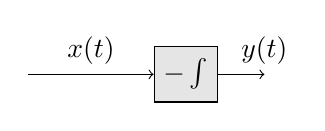
\begin{tikzpicture}[auto]
    \node [input, name=input] at (0,0) {};
    \node[block] at (2,0) (block1) {$-\int$};
    \node [output, right of=block1] (output) {};

    \draw [->] (input) -- node {$x(t)$} (block1);
    \draw [->] (block1) -- node[pos=1] {$y(t)$} (output);
  \end{tikzpicture}  

  &
    \begin{circuitikz}[american voltages,scale=0.8, every node/.style={transform shape}]
    \draw
    (5,3.5) node[op amp] (opamp1) {}
    (0,4) to[R,l=$R$,o-] (4,4)
    (4,4) to[short] (opamp1.-)
    (opamp1.+) to[short] (3.8,2) 
    (0,2) to[short,o-o] (8,2)
    (opamp1.out) to[short] (6.2,5)
    (3.5,5) to[C,l=$C$] (6.2,5)
    (3.5,4) to[short] (3.5,5)
    (opamp1.out) to[short,-o] (8,3.5)
    (0,4) to[open, v=$x(t)$] (0,2)
    (8,3.5) to[open, v=$y(t)$] (8,2);
    \end{circuitikz}\\
    \hline
\end{tabular}

\newpage
\subsection*{Solved Problems}

\begin{enumerate}
\item Consider a system with the following block diagram:
\begin{center}
  \tikzstyle{block} = [draw, fill=gray!20, rectangle, 
    minimum height=2em, minimum width=2em]
  \tikzstyle{sum} = [draw, fill=gray!20, circle, node distance=1cm]
  \tikzstyle{input} = [coordinate]
  \tikzstyle{output} = [coordinate]
  \tikzstyle{pinstyle} = [pin edge={to-,thin,black}]
  
  \begin{tikzpicture}[auto, node distance=2cm,>=latex',scale=1, every node/.style={transform shape}]
    \node [input, name=input] at (0,0) {};  	
    \node [block] at (4.5,0) (block1) {$\int$};
    \node [sum] at (2,0) (sum) {$\Sigma$};
    \node [output, name=feedback] at (6,0) {};  	
    \node [output, name=feedback2] at (6,1) {};  	
    \node [output, name=output] at (8,-5) {};  	
    \node [block] at (6,-2) (block2) {$\int$};
    \node [output, name=output2] at (6,-3) {};  	
    \node [block] at (6,-4) (block3) {$\int$};
    \node [output, name=output3] at (6,-5) {};  	
    \draw [->] (input) --  (sum);
    \draw [->] (sum) -- (block1);
    \draw (block1) -- (feedback);
    \draw (feedback) -- (feedback2);
    \draw [->] (feedback2) -| node[pos=0.95] {$-$} (sum);
    \draw [->] (output3) -- node {$b$} (output);
    \draw [->] (feedback) -- (block2);
    \draw [->] (block2) -- (block3);
    \draw [->] (output2) -| node[pos=0.95] {$-$} (sum);
    \draw (block3) -- (output3);
    \draw node at (-0.5,0) {$x(t)$};
    \draw node at (8.5,-5) {$y(t)$};
    \draw node at (4,-2.75) {$a$};
  \end{tikzpicture}
\end{center}

Determine the differential equation representation of this system.\\[1em]


\textbf{Solution:} We can convert this back to a differential equation representation as follows. First label the output of each block as a signal (called the internal states of the system), which we denote as $u(t)$, $v(t)$, $w(t)$, and $z(t)$ below.

\begin{center}
  \tikzstyle{block} = [draw, fill=gray!20, rectangle, 
    minimum height=2em, minimum width=2em]
  \tikzstyle{sum} = [draw, fill=gray!20, circle, node distance=1cm]
  \tikzstyle{input} = [coordinate]
  \tikzstyle{output} = [coordinate]
  \tikzstyle{pinstyle} = [pin edge={to-,thin,black}]
  
  \begin{tikzpicture}[auto, node distance=2cm,>=latex',scale=1, every node/.style={transform shape}]
    \node [input, name=input] at (0,0) {};  	
    \node [block] at (4.5,0) (block1) {$\int$};
    \node [sum] at (2,0) (sum) {$\Sigma$};
    \node [output, name=feedback] at (6,0) {};  	
    \node [output, name=feedback2] at (6,1) {};  	
    \node [output, name=output] at (8,-5) {};  	
    \node [block] at (6,-2) (block2) {$\int$};
    \node [output, name=output2] at (6,-3) {};  	
    \node [block] at (6,-4) (block3) {$\int$};
    \node [output, name=output3] at (6,-5) {};  	
    \draw [->] (input) --  (sum);
    \draw [->] (sum) -- (block1);
    \draw (block1) -- (feedback);
    \draw (feedback) -- (feedback2);
    \draw [->] (feedback2) -| node[pos=0.95] {$-$} (sum);
    \draw [->] (output3) -- node {$b$} (output);
    \draw [->] (feedback) -- (block2);
    \draw [->] (block2) -- (block3);
    \draw [->] (output2) -| node[pos=0.95] {$-$} (sum);
    \draw (block3) -- (output3);
    \draw node at (-0.5,0) {$x(t)$};
    \draw node at (8.5,-5) {$y(t)$};
    \draw node at (4,-2.75) {$a$};
    \draw node at (6.5,0) {$u(t)$};
    \draw node at (6.5,-3) {$v(t)$};
    \draw node at (3,-0.3) {$w(t)$};
    \draw node at (5.5,-5) {$z(t)$};
  \end{tikzpicture}
\end{center}
Now we can read off the input-output relationships moving from input to output. Starting with the output of the summation
\[
w(t) = x(t) - u(t) -a\,v(t) \; .
\]
The outputs of each integrator are:
\[
u(t) = \int\limits_{-\infty}^t w(\tau) \; d\tau\;, \;
v(t) = \int\limits_{-\infty}^t u(\tau) \; d\tau\;, \mbox{ and }\;
z(t) = \int\limits_{-\infty}^t v(\tau) \; d\tau
\]
or equivalently
\[
\frac{du}{dt}(t) = w(t)\;,\; \frac{dv}{dt}(t) = u(t)\; ,\; \mbox{ and }\; \frac{dz}{dt}(t) = v(t)
\]
Finally, the output is:
\[
y(t) = b\, z(t)\; .
\]
We now do a series of derivatives and substitutions
\begin{align*}
  y(t) &= b\, z(t)\\
  \frac{dy}{dt}(t) &= b\, \frac{dz}{dt}(t)\\
  &= b\, v(t)\\
  \frac{d^2y}{dt^2}(t) &= b\, \frac{dv}{dt}(t)\\
  &= b\, u(t)\\
  \frac{d^3y}{dt^3}(t) &= b\, \frac{du}{dt}(t)\\
  &= b\, w(t)\\
  &= b\left( x(t) - u(t) -a\,v(t)\right)
\end{align*}
Rearranging the last equation to isolate the input on the right hand side gives
\[
\frac{d^3y}{dt^3}(t) + b\,u(t) +ab\,v(t) = b\,x(t)\; \mbox{ (Eqn.~1)}
\]
We can now note from above
\[
u(t) = \frac{dv}{dt}(t) =  \frac{d^2z}{dt^2}(t) = \frac{1}{b} \frac{d^2y}{dt^2}(t) \mbox{ and }
\]
\[
v(t) = \frac{dz}{dt}(t) = \frac{1}{b} \frac{dy}{dt}(t)\; .
\]
Substituting these back into Eqn.~1 gives
\[
\frac{d^3y}{dt^3}(t) + \frac{d^2y}{dt^2}(t) +a\,\frac{dy}{dt}(t) = b\,x(t)
\]
Which is a LCCDE.\\
$\blacksquare$
\end{enumerate}

